%%%%%%%%%%%%%%%%%%%%%%%%%%%%%%%%%%%%%%%%%
% The Legrand Orange Book
% LaTeX Template
% Version 2.1.1 (14/2/16)
%
% This template has been downloaded from:
% http://www.LaTeXTemplates.com
%
% Original author:
% Mathias Legrand (legrand.mathias@gmail.com) with modifications by:
% Vel (vel@latextemplates.com)
%
% License:
% CC BY-NC-SA 3.0 (http://creativecommons.org/licenses/by-nc-sa/3.0/)
%
% Compiling this template:
% This template uses biber for its bibliography and makeindex for its index.
% When you first open the template, compile it from the command line with the 
% commands below to make sure your LaTeX distribution is configured correctly:
%
% 1) pdflatex main
% 2) makeindex main.idx -s StyleInd.ist
% 3) biber main
% 4) pdflatex main x 2
%
% After this, when you wish to update the bibliography/index use the appropriate
% command above and make sure to compile with pdflatex several times 
% afterwards to propagate your changes to the document.
%
% This template also uses a number of packages which may need to be
% updated to the newest versions for the template to compile. It is strongly
% recommended you update your LaTeX distribution if you have any
% compilation errors.
%
% Important note:
% Chapter heading images should have a 2:1 width:height ratio,
% e.g. 920px width and 460px height.
%
%%%%%%%%%%%%%%%%%%%%%%%%%%%%%%%%%%%%%%%%%

%----------------------------------------------------------------------------------------
%	PACKAGES AND OTHER DOCUMENT CONFIGURATIONS
%----------------------------------------------------------------------------------------

\documentclass[11pt,openany]{book} % Default font size and left-justified equations

%----------------------------------------------------------------------------------------

%%%%%%%%%%%%%%%%%%%%%%%%%%%%%%%%%%%%%%%%%
% The Legrand Orange Book
% Structural Definitions File
% Version 2.0 (9/2/15)
%
% Original author:
% Mathias Legrand (legrand.mathias@gmail.com) with modifications by:
% Vel (vel@latextemplates.com)
% 
% This file has been downloaded from:
% http://www.LaTeXTemplates.com
%
% License:
% CC BY-NC-SA 3.0 (http://creativecommons.org/licenses/by-nc-sa/3.0/)
%
%%%%%%%%%%%%%%%%%%%%%%%%%%%%%%%%%%%%%%%%%

%----------------------------------------------------------------------------------------
%   VARIOUS REQUIRED PACKAGES AND CONFIGURATIONS
%----------------------------------------------------------------------------------------

\usepackage[top=3cm,bottom=3cm,left=3cm,right=3cm,headsep=10pt,a4paper]{geometry} % Page margins

\usepackage[table]{xcolor}% Required for specifying colors by name
\usepackage{graphicx} % Required for including pictures
\graphicspath{{Pictures/}} % Specifies the directory where pictures are stored

\usepackage{lipsum} % Inserts dummy text

\usepackage{tikz} % Required for drawing custom shapes

\usepackage[spanish]{babel} % English language/hyphenation

% \usepackage{enumitem} % Customize lists
\usepackage{enumerate}
% \setlist{nolistsep} % Reduce spacing between bullet points and numbered lists

\usepackage{booktabs} % Required for nicer horizontal rules in tables

% \definecolor{ocre}{RGB}{243,102,25} % Define the orange color used for highlighting throughout the book
\definecolor{ocre}{rgb}{0.0, 0.5, 1.0}

%----------------------------------------------------------------------------------------
%	FONTS
%----------------------------------------------------------------------------------------

\usepackage{avant} % Use the Avantgarde font for headings
%\usepackage{times} % Use the Times font for headings
\usepackage{mathptmx} % Use the Adobe Times Roman as the default text font together with math symbols from the Sym­bol, Chancery and Com­puter Modern fonts

\usepackage{microtype} % Slightly tweak font spacing for aesthetics
\usepackage[utf8]{inputenc} % Required for including letters with accents
\usepackage[T1]{fontenc} % Use 8-bit encoding that has 256 glyphs

% \usepackage{minted}

%----------------------------------------------------------------------------------------
%	BIBLIOGRAPHY AND INDEX
%----------------------------------------------------------------------------------------

\usepackage[style=alphabetic,citestyle=numeric,sorting=nyt,sortcites=true,autopunct=true,babel=hyphen,hyperref=true,abbreviate=false,backref=true,backend=biber]{biblatex}
\addbibresource{bibliography.bib} % BibTeX bibliography file
\defbibheading{bibempty}{}

\usepackage{calc} % For simpler calculation - used for spacing the index letter headings correctly
\usepackage{makeidx} % Required to make an index
\makeindex % Tells LaTeX to create the files required for indexing

%----------------------------------------------------------------------------------------
%	MAIN TABLE OF CONTENTS
%----------------------------------------------------------------------------------------

\usepackage{titletoc} % Required for manipulating the table of contents

\contentsmargin{0cm} % Removes the default margin

% Part text styling
\titlecontents{part}[0cm]
{\addvspace{20pt}\centering\large\bfseries}
{}
{}
{}

% Chapter text styling
\titlecontents{chapter}[1.25cm] % Indentation
{\addvspace{12pt}\large\sffamily\bfseries} % Spacing and font options for chapters
{\color{ocre!60}\contentslabel[\Large\thecontentslabel]{1.25cm}\color{ocre}} % Chapter number
{\color{ocre}}  
{\color{ocre!60}\normalsize\;\titlerule*[.5pc]{.}\;\thecontentspage} % Page number

% Section text styling
\titlecontents{section}[1.25cm] % Indentation
{\addvspace{3pt}\sffamily\bfseries} % Spacing and font options for sections
{\contentslabel[\thecontentslabel]{1.25cm}} % Section number
{}
{\hfill\color{black}\thecontentspage} % Page number
[]

% Subsection text styling
\titlecontents{subsection}[1.25cm] % Indentation
{\addvspace{1pt}\sffamily\small} % Spacing and font options for subsections
{\contentslabel[\thecontentslabel]{1.25cm}} % Subsection number
{}
{\ \titlerule*[.5pc]{.}\;\thecontentspage} % Page number
[]

% List of figures
\titlecontents{figure}[0em]
{\addvspace{-5pt}\sffamily}
{\thecontentslabel\hspace*{1em}}
{}
{\ \titlerule*[.5pc]{.}\;\thecontentspage}
[]

% List of tables
\titlecontents{table}[0em]
{\addvspace{-5pt}\sffamily}
{\thecontentslabel\hspace*{1em}}
{}
{\ \titlerule*[.5pc]{.}\;\thecontentspage}
[]

%----------------------------------------------------------------------------------------
%	MINI TABLE OF CONTENTS IN PART HEADS
%----------------------------------------------------------------------------------------

% Chapter text styling
\titlecontents{lchapter}[0em] % Indenting
{\addvspace{15pt}\large\sffamily\bfseries} % Spacing and font options for chapters
{\color{ocre}\contentslabel[\Large\thecontentslabel]{1.25cm}\color{ocre}} % Chapter number
{}  
{\color{ocre}\normalsize\sffamily\bfseries\;\titlerule*[.5pc]{.}\;\thecontentspage} % Page number

% Section text styling
\titlecontents{lsection}[0em] % Indenting
{\sffamily\small} % Spacing and font options for sections
{\contentslabel[\thecontentslabel]{1.25cm}} % Section number
{}
{}

% Subsection text styling
\titlecontents{lsubsection}[.5em] % Indentation
{\normalfont\footnotesize\sffamily} % Font settings
{}
{}
{}

%----------------------------------------------------------------------------------------
%	PAGE HEADERS
%----------------------------------------------------------------------------------------

\usepackage{fancyhdr} % Required for header and footer configuration

\pagestyle{fancy}
\renewcommand{\chaptermark}[1]{\markboth{\sffamily\normalsize\bfseries\chaptername\ \thechapter.\ #1}{}} % Chapter text font settings
\renewcommand{\sectionmark}[1]{\markright{\sffamily\normalsize\thesection\hspace{5pt}#1}{}} % Section text font settings
\fancyhf{} \fancyhead[LE,RO]{\sffamily\normalsize\thepage} % Font setting for the page number in the header
\fancyhead[LO]{\rightmark} % Print the nearest section name on the left side of odd pages
\fancyhead[RE]{\leftmark} % Print the current chapter name on the right side of even pages
\renewcommand{\headrulewidth}{0.5pt} % Width of the rule under the header
\addtolength{\headheight}{2.5pt} % Increase the spacing around the header slightly
\renewcommand{\footrulewidth}{0pt} % Removes the rule in the footer
\fancypagestyle{plain}{\fancyhead{}\renewcommand{\headrulewidth}{0pt}} % Style for when a plain pagestyle is specified

% Removes the header from odd empty pages at the end of chapters
\makeatletter
\renewcommand{\cleardoublepage}{
\clearpage\ifodd\c@page\else
\hbox{}
\vspace*{\fill}
\thispagestyle{empty}
\newpage
\fi}

%----------------------------------------------------------------------------------------
%	THEOREM STYLES
%----------------------------------------------------------------------------------------

\usepackage{amsmath,amsfonts,amssymb,amsthm} % For math equations, theorems, symbols, etc

\newcommand{\intoo}[2]{\mathopen{]}#1\,;#2\mathclose{[}}
\newcommand{\ud}{\mathop{\mathrm{{}d}}\mathopen{}}
\newcommand{\intff}[2]{\mathopen{[}#1\,;#2\mathclose{]}}
\newtheorem{notation}{Notation}[chapter]

% Boxed/framed environments
\newtheoremstyle{ocrenumbox}% % Theorem style name
{0pt}% Space above
{0pt}% Space below
{\normalfont}% % Body font
{}% Indent amount
{\small\bf\sffamily\color{ocre}}% % Theorem head font
{\;}% Punctuation after theorem head
{0.25em}% Space after theorem head
{\small\sffamily\color{ocre}\thmname{#1}\nobreakspace\thmnumber{\@ifnotempty{#1}{}\@upn{#2}}% Theorem text (e.g. Theorem 2.1)
\thmnote{\nobreakspace\the\thm@notefont\sffamily\bfseries\color{black}---\nobreakspace#3.}} % Optional theorem note
\renewcommand{\qedsymbol}{$\blacksquare$}% Optional qed square

\newtheoremstyle{blacknumex}% Theorem style name
{5pt}% Space above
{5pt}% Space below
{\normalfont}% Body font
{} % Indent amount
{\small\bf\sffamily}% Theorem head font
{\;}% Punctuation after theorem head
{0.25em}% Space after theorem head
{\small\sffamily{\tiny\ensuremath{\blacksquare}}\nobreakspace\thmname{#1}\nobreakspace\thmnumber{\@ifnotempty{#1}{}\@upn{#2}}% Theorem text (e.g. Theorem 2.1)
\thmnote{\nobreakspace\the\thm@notefont\sffamily\bfseries---\nobreakspace#3.}}% Optional theorem note

\newtheoremstyle{blacknumbox} % Theorem style name
{0pt}% Space above
{0pt}% Space below
{\normalfont}% Body font
{}% Indent amount
{\small\bf\sffamily}% Theorem head font
{\;}% Punctuation after theorem head
{0.25em}% Space after theorem head
{\small\sffamily\thmname{#1}\nobreakspace\thmnumber{\@ifnotempty{#1}{}\@upn{#2}}% Theorem text (e.g. Theorem 2.1)
\thmnote{\nobreakspace\the\thm@notefont\sffamily\bfseries---\nobreakspace#3.}}% Optional theorem note

% Non-boxed/non-framed environments
\newtheoremstyle{ocrenum}% % Theorem style name
{5pt}% Space above
{5pt}% Space below
{\normalfont}% % Body font
{}% Indent amount
{\small\bf\sffamily\color{ocre}}% % Theorem head font
{\;}% Punctuation after theorem head
{0.25em}% Space after theorem head
{\small\sffamily\color{ocre}\thmname{#1}\nobreakspace\thmnumber{\@ifnotempty{#1}{}\@upn{#2}}% Theorem text (e.g. Theorem 2.1)
\thmnote{\nobreakspace\the\thm@notefont\sffamily\bfseries\color{black}---\nobreakspace#3.}} % Optional theorem note
\renewcommand{\qedsymbol}{$\blacksquare$}% Optional qed square
\makeatother

% Defines the theorem text style for each type of theorem to one of the three styles above
\newcounter{dummy} 
\numberwithin{dummy}{section}
\theoremstyle{ocrenumbox}
\newtheorem{theoremeT}[dummy]{Fórmula}
\newtheorem{problem}{Problem}[chapter]
\newtheorem{exerciseT}{Exercise}[chapter]
\theoremstyle{blacknumex}
\newtheorem{exampleT}{Example}[chapter]
\theoremstyle{blacknumbox}
\newtheorem{vocabulary}{Vocabulary}[chapter]
\newtheorem{definitionT}{Definition}[section]
\newtheorem{corollaryT}[dummy]{Corollary}
\theoremstyle{ocrenum}
\newtheorem{proposition}[dummy]{Proposition}

%----------------------------------------------------------------------------------------
%	DEFINITION OF COLORED BOXES
%----------------------------------------------------------------------------------------

\RequirePackage[framemethod=default]{mdframed} % Required for creating the theorem, definition, exercise and corollary boxes

% Theorem box
\newmdenv[skipabove=7pt,
skipbelow=7pt,
backgroundcolor=black!5,
linecolor=ocre,
innerleftmargin=5pt,
innerrightmargin=5pt,
innertopmargin=5pt,
leftmargin=0cm,
rightmargin=0cm,
innerbottommargin=5pt]{tBox}

% Exercise box	  
\newmdenv[skipabove=7pt,
skipbelow=7pt,
rightline=false,
leftline=true,
topline=false,
bottomline=false,
backgroundcolor=ocre!10,
linecolor=ocre,
innerleftmargin=5pt,
innerrightmargin=5pt,
innertopmargin=5pt,
innerbottommargin=5pt,
leftmargin=0cm,
rightmargin=0cm,
linewidth=4pt]{eBox}	

% Definition box
\newmdenv[skipabove=7pt,
skipbelow=7pt,
rightline=false,
leftline=true,
topline=false,
bottomline=false,
linecolor=ocre,
innerleftmargin=5pt,
innerrightmargin=5pt,
innertopmargin=0pt,
leftmargin=0cm,
rightmargin=0cm,
linewidth=4pt,
innerbottommargin=0pt]{dBox}	

% Corollary box
\newmdenv[skipabove=7pt,
skipbelow=7pt,
rightline=false,
leftline=true,
topline=false,
bottomline=false,
linecolor=gray,
backgroundcolor=black!5,
innerleftmargin=5pt,
innerrightmargin=5pt,
innertopmargin=5pt,
leftmargin=0cm,
rightmargin=0cm,
linewidth=4pt,
innerbottommargin=5pt]{cBox}

% Creates an environment for each type of theorem and assigns it a theorem text style from the "Theorem Styles" section above and a colored box from above
\newenvironment{theorem}{\begin{tBox}\begin{theoremeT}}{\end{theoremeT}\end{tBox}}
\newenvironment{exercise}{\begin{eBox}\begin{exerciseT}}{\hfill{\color{ocre}\tiny\ensuremath{\blacksquare}}\end{exerciseT}\end{eBox}}				  
\newenvironment{definition}{\begin{dBox}\begin{definitionT}}{\end{definitionT}\end{dBox}}	
\newenvironment{example}{\begin{exampleT}}{\hfill{\tiny\ensuremath{\blacksquare}}\end{exampleT}}		
\newenvironment{corollary}{\begin{cBox}\begin{corollaryT}}{\end{corollaryT}\end{cBox}}	

%----------------------------------------------------------------------------------------
%	REMARK ENVIRONMENT
%----------------------------------------------------------------------------------------

\newenvironment{remark}{\par\vspace{10pt}\small % Vertical white space above the remark and smaller font size
\begin{list}{}{
\leftmargin=35pt % Indentation on the left
\rightmargin=25pt}\item\ignorespaces % Indentation on the right
\makebox[-2.5pt]{\begin{tikzpicture}[overlay]
\node[draw=ocre!60,line width=1pt,circle,fill=ocre!25,font=\sffamily\bfseries,inner sep=2pt,outer sep=0pt] at (-15pt,0pt){\textcolor{ocre}{R}};\end{tikzpicture}} % Orange R in a circle
\advance\baselineskip -1pt}{\end{list}\vskip5pt} % Tighter line spacing and white space after remark

%----------------------------------------------------------------------------------------
%	SECTION NUMBERING IN THE MARGIN
%----------------------------------------------------------------------------------------

\makeatletter
\renewcommand{\@seccntformat}[1]{\llap{\textcolor{ocre}{\csname the#1\endcsname}\hspace{1em}}}                    
\renewcommand{\section}{\@startsection{section}{1}{\z@}
{-4ex \@plus -1ex \@minus -.4ex}
{1ex \@plus.2ex }
{\normalfont\large\sffamily\bfseries}}
\renewcommand{\subsection}{\@startsection {subsection}{2}{\z@}
{-3ex \@plus -0.1ex \@minus -.4ex}
{0.5ex \@plus.2ex }
{\normalfont\sffamily\bfseries}}
\renewcommand{\subsubsection}{\@startsection {subsubsection}{3}{\z@}
{-2ex \@plus -0.1ex \@minus -.2ex}
{.2ex \@plus.2ex }
{\normalfont\small\sffamily\bfseries}}                        
\renewcommand\paragraph{\@startsection{paragraph}{4}{\z@}
{-2ex \@plus-.2ex \@minus .2ex}
{.1ex}
{\normalfont\small\sffamily\bfseries}}

%----------------------------------------------------------------------------------------
%	PART HEADINGS
%----------------------------------------------------------------------------------------

% numbered part in the table of contents
\newcommand{\@mypartnumtocformat}[2]{%
\setlength\fboxsep{0pt}%
\noindent\colorbox{ocre!20}{\strut\parbox[c][.7cm]{\ecart}{\color{ocre!70}\Large\sffamily\bfseries\centering#1}}\hskip\esp\colorbox{ocre!40}{\strut\parbox[c][.7cm]{\linewidth-\ecart-\esp}{\Large\sffamily\centering#2}}}%
%%%%%%%%%%%%%%%%%%%%%%%%%%%%%%%%%%
% unnumbered part in the table of contents
\newcommand{\@myparttocformat}[1]{%
\setlength\fboxsep{0pt}%
\noindent\colorbox{ocre!40}{\strut\parbox[c][.7cm]{\linewidth}{\Large\sffamily\centering#1}}}%
%%%%%%%%%%%%%%%%%%%%%%%%%%%%%%%%%%
\newlength\esp
\setlength\esp{4pt}
\newlength\ecart
\setlength\ecart{1.2cm-\esp}
\newcommand{\thepartimage}{}%
\newcommand{\partimage}[1]{\renewcommand{\thepartimage}{#1}}%
\def\@part[#1]#2{%
\ifnum \c@secnumdepth >-2\relax%
\refstepcounter{part}%
\addcontentsline{toc}{part}{\texorpdfstring{\protect\@mypartnumtocformat{\thepart}{#1}}{\partname~\thepart\ ---\ #1}}
\else%
\addcontentsline{toc}{part}{\texorpdfstring{\protect\@myparttocformat{#1}}{#1}}%
\fi%
\startcontents%
\markboth{}{}%
{\thispagestyle{empty}%
\begin{tikzpicture}[remember picture,overlay]%
\node at (current page.north west){\begin{tikzpicture}[remember picture,overlay]%	
\fill[ocre!20](0cm,0cm) rectangle (\paperwidth,-\paperheight);
\node[anchor=north] at (4cm,-3.25cm){\color{ocre!40}\fontsize{220}{100}\sffamily\bfseries\@Roman\c@part}; 
\node[anchor=south east] at (\paperwidth-1cm,-\paperheight+1cm){\parbox[t][][t]{8.5cm}{
\printcontents{l}{0}{\setcounter{tocdepth}{1}}%
}};
\node[anchor=north east] at (\paperwidth-1.5cm,-3.25cm){\parbox[t][][t]{15cm}{\strut\raggedleft\color{white}\fontsize{30}{30}\sffamily\bfseries#2}};
\end{tikzpicture}};
\end{tikzpicture}}%
\@endpart}
\def\@spart#1{%
\startcontents%
\phantomsection
{\thispagestyle{empty}%
\begin{tikzpicture}[remember picture,overlay]%
\node at (current page.north west){\begin{tikzpicture}[remember picture,overlay]%	
\fill[ocre!20](0cm,0cm) rectangle (\paperwidth,-\paperheight);
\node[anchor=north east] at (\paperwidth-1.5cm,-3.25cm){\parbox[t][][t]{15cm}{\strut\raggedleft\color{white}\fontsize{30}{30}\sffamily\bfseries#1}};
\end{tikzpicture}};
\end{tikzpicture}}
\addcontentsline{toc}{part}{\texorpdfstring{%
\setlength\fboxsep{0pt}%
\noindent\protect\colorbox{ocre!40}{\strut\protect\parbox[c][.7cm]{\linewidth}{\Large\sffamily\protect\centering #1\quad\mbox{}}}}{#1}}%
\@endpart}
\def\@endpart{\vfil\newpage
\if@twoside
\if@openright
\null
\thispagestyle{empty}%
\newpage
\fi
\fi
\if@tempswa
\twocolumn
\fi}

%----------------------------------------------------------------------------------------
%	CHAPTER HEADINGS
%----------------------------------------------------------------------------------------

% A switch to conditionally include a picture, implemented by  Christian Hupfer
\newif\ifusechapterimage
\usechapterimagetrue
\newcommand{\thechapterimage}{}%
\newcommand{\chapterimage}[1]{\ifusechapterimage\renewcommand{\thechapterimage}{#1}\fi}%
\def\@makechapterhead#1{%
{\parindent \z@ \raggedright \normalfont
\ifnum \c@secnumdepth >\m@ne
\if@mainmatter
\begin{tikzpicture}[remember picture,overlay]
\node at (current page.north west)
{\begin{tikzpicture}[remember picture,overlay]
\node[anchor=north west,inner sep=0pt] at (0,0) {\ifusechapterimage\includegraphics[width=\paperwidth]{\thechapterimage}\fi};
\draw[anchor=west] (\Gm@lmargin,-9cm) node [line width=2pt,rounded corners=15pt,draw=ocre,fill=white,fill opacity=0.5,inner sep=15pt]{\strut\makebox[22cm]{}};
\draw[anchor=west] (\Gm@lmargin+.3cm,-9cm) node {\huge\sffamily\bfseries\color{black}\thechapter. #1\strut};
\end{tikzpicture}};
\end{tikzpicture}
\else
\begin{tikzpicture}[remember picture,overlay]
\node at (current page.north west)
{\begin{tikzpicture}[remember picture,overlay]
\node[anchor=north west,inner sep=0pt] at (0,0) {\ifusechapterimage\includegraphics[width=\paperwidth]{\thechapterimage}\fi};
\draw[anchor=west] (\Gm@lmargin,-9cm) node [line width=2pt,rounded corners=15pt,draw=ocre,fill=white,fill opacity=0.5,inner sep=15pt]{\strut\makebox[22cm]{}};
\draw[anchor=west] (\Gm@lmargin+.3cm,-9cm) node {\huge\sffamily\bfseries\color{black}#1\strut};
\end{tikzpicture}};
\end{tikzpicture}
\fi\fi\par\vspace*{270\p@}}}

%-------------------------------------------

\def\@makeschapterhead#1{%
\begin{tikzpicture}[remember picture,overlay]
\node at (current page.north west)
{\begin{tikzpicture}[remember picture,overlay]
\node[anchor=north west,inner sep=0pt] at (0,0) {\ifusechapterimage\includegraphics[width=\paperwidth]{\thechapterimage}\fi};
\draw[anchor=west] (\Gm@lmargin,-9cm) node [line width=2pt,rounded corners=15pt,draw=ocre,fill=white,fill opacity=0.5,inner sep=15pt]{\strut\makebox[22cm]{}};
\draw[anchor=west] (\Gm@lmargin+.3cm,-9cm) node {\huge\sffamily\bfseries\color{black}#1\strut};
\end{tikzpicture}};
\end{tikzpicture}
\par\vspace*{270\p@}}
\makeatother

%----------------------------------------------------------------------------------------
%	HYPERLINKS IN THE DOCUMENTS
%----------------------------------------------------------------------------------------

\usepackage{hyperref}
\hypersetup{hidelinks,backref=true,pagebackref=true,hyperindex=true,colorlinks=false,breaklinks=true,urlcolor= ocre,bookmarks=true,bookmarksopen=false,pdftitle={Sistema experto en CLIPS para asesorar a un inversor en bolsa},pdfauthor={Marta Gómez Macías}}
\usepackage{bookmark}
\bookmarksetup{
open,
numbered,
addtohook={%
\ifnum\bookmarkget{level}=0 % chapter
\bookmarksetup{bold}%
\fi
\ifnum\bookmarkget{level}=-1 % part
\bookmarksetup{color=ocre,bold}%
\fi
}
}
 % Insert the commands.tex file which contains the majority of the structure behind the template

\setlength{\parindent}{0pt}
\setlength{\parskip}{1ex plus 0.5ex minus 0.2ex}


\begin{document}
\renewcommand{\tablename}{Tabla} 
%----------------------------------------------------------------------------------------
%	TITLE PAGE
%----------------------------------------------------------------------------------------

\begingroup
\thispagestyle{empty}
\begin{tikzpicture}[remember picture,overlay]
\coordinate [below=12cm] (midpoint) at (current page.north);
\node at (current page.north west)
{\begin{tikzpicture}[remember picture,overlay]
\node[anchor=north west,inner sep=0pt] at (0,0) {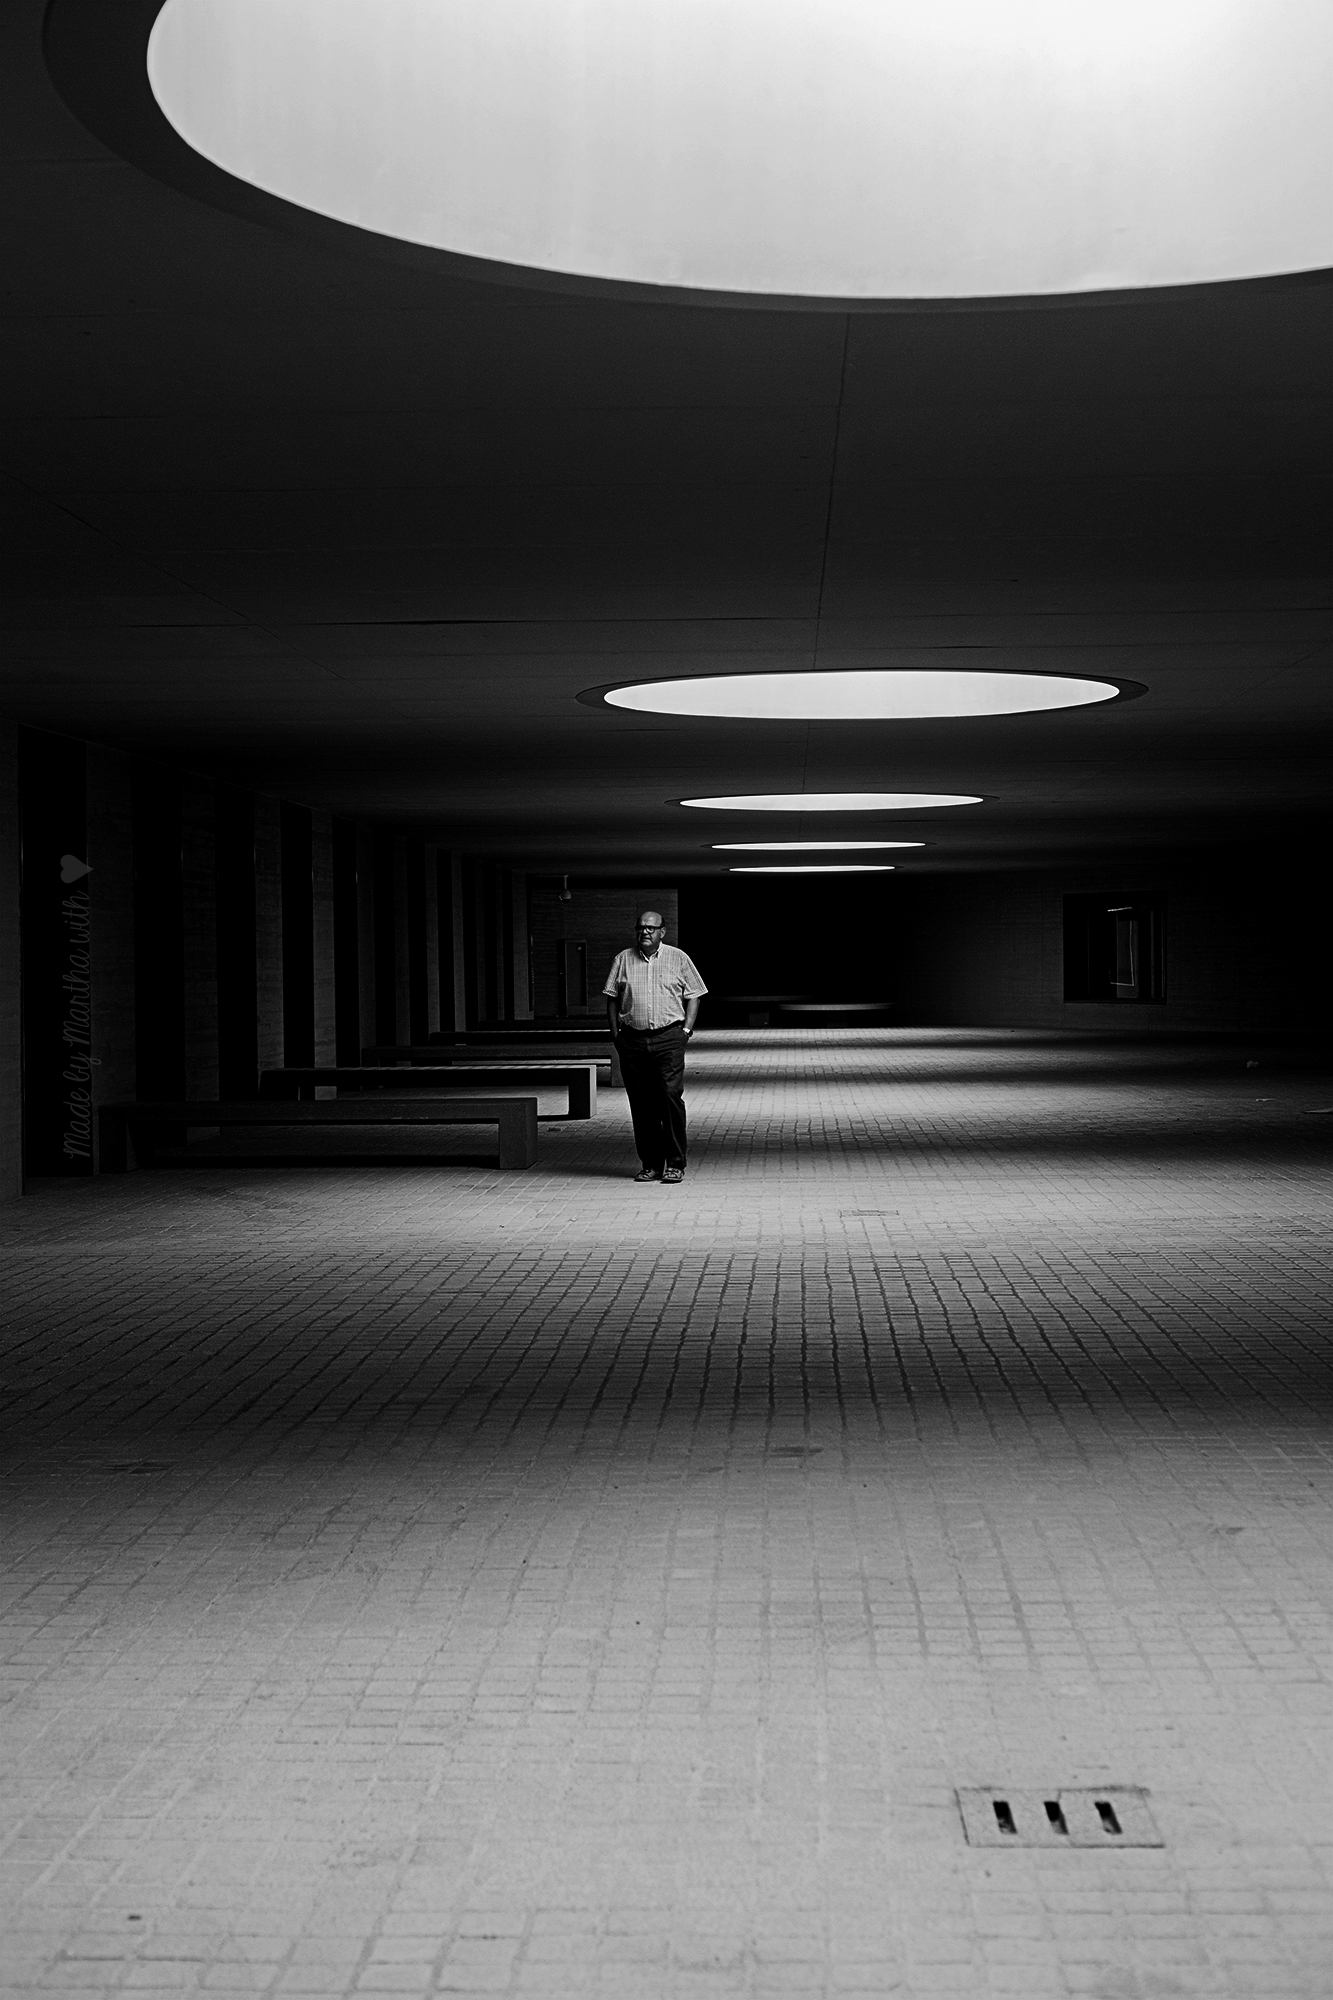
\includegraphics[width=\paperwidth]{background}}; % Background image
\node[anchor=north] (box) at (10,-20.5) [fill=ocre!30!white,fill opacity=0.6,text opacity=1,inner sep=1cm]{\Huge\centering\bfseries\sffamily\parbox[c][][t]{\paperwidth}{\centering Sistema experto en CLIPS\\ para asesorar a un inversor en bolsa \\[15pt] % Book title
{\Large Universidad de Granada}\\[20pt] % Subtitle
{\huge Marta Gómez Macías - 75929776Z}}}; % Author name
\end{tikzpicture}};
\end{tikzpicture}
\vfill
\endgroup

%----------------------------------------------------------------------------------------
%	COPYRIGHT PAGE
%----------------------------------------------------------------------------------------

% \newpage
% ~\vfill
% \thispagestyle{empty}

% \noindent Copyright \copyright\ 2013 John Smith\\ % Copyright notice

% \noindent \textsc{Published by Publisher}\\ % Publisher

% \noindent \textsc{book-website.com}\\ % URL

% \noindent Licensed under the Creative Commons Attribution-NonCommercial 3.0 Unported License (the ``License''). You may not use this file except in compliance with the License. You may obtain a copy of the License at \url{http://creativecommons.org/licenses/by-nc/3.0}. Unless required by applicable law or agreed to in writing, software distributed under the License is distributed on an \textsc{``as is'' basis, without warranties or conditions of any kind}, either express or implied. See the License for the specific language governing permissions and limitations under the License.\\ % License information

% \noindent \textit{First printing, March 2013} % Printing/edition date

%----------------------------------------------------------------------------------------
%	TABLE OF CONTENTS
%----------------------------------------------------------------------------------------

%\usechapterimagefalse % If you don't want to include a chapter image, use this to toggle images off - it can be enabled later with \usechapterimagetrue

\chapterimage{chapter_head_1} % Table of contents heading image

\pagestyle{empty} % No headers

\tableofcontents % Print the table of contents itself

% \cleardoublepage % Forces the first chapter to start on an odd page so it's on the right

\pagestyle{fancy} % Print headers again

%----------------------------------------------------------------------------------------
%	PART
%----------------------------------------------------------------------------------------

% \part{Part One}

%----------------------------------------------------------------------------------------
%	CHAPTER 1
%----------------------------------------------------------------------------------------

\chapterimage{chapter_head_2} % Chapter heading image

\chapter{Resumen del comportamiento del S.E.}

En primer lugar, el sistema experto comienza leyendo la información sobre las empresas del Ibex 35, los sectores y las noticias. También lee la cartera del usuario. Una vez tiene todo almacenado en memoria, comienza a deducir valores:

\begin{enumerate}[\qquad\color{ocre}{$\bullet$}]
    \item En primer lugar, deduce \textit{\textcolor{ocre}{valores inestables}} basándose en el sector de la empresa y las noticias negativas.
    \item Después,  los \textit{\textcolor{ocre}{valores estables}} basándose en las noticias positivas.
    \item Basándose en los valores inestables calculados anteriormente, calcula los \textit{\textcolor{ocre}{valores peligrosos}}, aunque sólo realiza dicho cálculo con los valores que están en la cartera del usuario.
    \item Una vez hecho esto, pasa a calcular los \textit{\textcolor{ocre}{valores sobrevalorados}} basándose en su \textbf{\textcolor{ocre}{PER}}\footnote{Price-to-Earnings Ratio} y en su \textbf{\textcolor{ocre}{RPD}}\footnote{Rentabilidad Por Dividendo} y el tamaño de la empresa 
    \item Por último, el sistema calcula los \textit{\textcolor{ocre}{valores infravalorados}}, basándose en el \textbf{\textcolor{ocre}{PER}} y la variación del precio de las acciones.
\end{enumerate}

Una vez ha calculado los distintos valores, pasa a buscar propuestas para presentar al usuario.

Tras obtener propuestas para el usuario, el sistema escoge las cinco mejores, es decir, las que tengan un mayor Rendimiento Esperado y se las presenta al usuario. El usuario escoge una de esas cinco y el sistema, tras la selección del usuario, actualiza su cartera y vuelve a calcular nuevas propuestas. Este paso se repite hasta que el usuario decide salir del programa.

\chapterimage{chapter_head_3}

\chapter{Descripción del proceso de desarrollo}

\section{Sesiones con el experto e información obtenida en cada una}
Antes de la primera sesión, estuve ojeando un artículo sobre inversión en bolsa y apunté los conceptos de los que se hablaba, para después preguntar al experto. Esta sesión la preparé así para ir familiarizándome con los conceptos de los que hablaría más tarde con el experto. Ya en dicha sesión, estuve hablando con el experto, con el director del proyecto y con el usuario final. 

Respecto al \textit{\textcolor{ocre}{usuario final}}, dijo que no le importaba introducir a mano su cartera y las noticias positivas y negativas sobre las empresas del sector. El \textit{\textcolor{ocre}{director}}, explicó cómo quería que fuese el proyecto y el objetivo final de éste, asesorar a inversores en bolsa novatos. También explicó la funcionalidad deseada que quería: que el sistema obtuviese cinco propuestas y dejase al usuario elegir una de ellas, una vez elegida una el sistema debería volver a mostrar nuevas opciones hasta que el usuario cerrase el programa. Por último, el \textit{\textcolor{ocre}{experto}} comentó los conceptos básicos que yo le pregunté y dio unas pautas muy generales sobre su método para invertir.

Las siguientes reuniones se hicieron sólo con el experto, y se fue profundizando en el proceso que éste realiza para invertir. En la segunda reunión, se estuvo hablando de los distintos pasos que el experto aplica, y que finalmente han sido los módulos del sistema. No se llegó a entrar en mucho detalle en cada uno de los pasos. En la última reunión, sí que describimos con detalle cada uno de los pasos que el experto realiza. Tras ésta última reunión, elaboré un documento con todas las reglas que el experto dijo y nos vimos una vez más para aclarar conceptos que habían quedado algo ambigüos. 

\section{Procedimiento de validación y verificación del sistema seguido}

Mientras iba desarrollando el sistema, fui probando cada regla para ver que funcionaba correctamente y se lanzaba cuando tenía que hacerlo. Una vez terminé de desarrollar el sistema, probé en primer lugar que la interfaz de usuario funcionase correctamente. Para ello, ejecuté el programa y probé con las distintas opciones que ofrecía, a ver si alguna no funcionaba. Efectivamente, me encontré fallos, sobre todo a la hora de salir del programa. Una vez la interfaz funcionó, comprobé que los resultados que daba el programa eran lógicos y estaban bien calculados.

Lo que he visto en relación a esto último, es que cuando el sistema te ofrece varias opciones y se escoge una distinta de la que tiene el máximo Rendimiento Esperado, el sistema puede ofrecerte, en la siguiente serie de propuestas, deshacer esa opción que escogiste. No sé si esto puede llegar a ser correcto o no, pues no es lógico hacer una cosa y después deshacerla. Le pregunté al experto y éste dijo que sí era normal hacer estas propuestas y que, como se presentan cinco propuestas diferentes al usuario, éste puede esoger cualquier otra.

\chapterimage{chapter_head_4}
\chapter{Descripción del sistema desarrollado}

\section{Variables de entrada del problema}

El problema tiene cuatro variables de entrada, que son:

\begin{enumerate}[\color{ocre}{$\bullet$}]
    \item \textit{\textbf{\textcolor{ocre}{Empresas del Ibex 35}}}: el usuario tiene almacenados en un fichero datos sobre las empresas del Ibex 35. El programa se encarga de leer el fichero y crear una variable \texttt{\textcolor{ocre}{ValorEmpresaIbex35}} por cada empresa con los siguientes campos de la \hyperref[valorempresaibex]{Tabla \ref*{valorempresaibex}}

    \begin{table}[!h]
    \centering
    {\rowcolors{2}{white!80!ocre!50}{ocre!70!white!40}
    \begin{tabular}{|c|p{8cm}|}
    \hline
    \textcolor{ocre}{\textit{\textbf{Variable}}} & \textcolor{ocre}{\textit{\textbf{Explicación}}} \\
    \hline
    \textit{Nombre} & Nombre de la empresa \\
    \hline
    \textit{Precio} & Precio en euros de una acción de la empresa \\
    \hline
    \textit{Variación Diaria} & Porcentaje de variación del precio respecto al cierre de la sesión anterior \\
    \hline
    \textit{Capitalización} & Valor total de la empresa: $precio \cdot num\;acciones$\\
    \hline
    \textit{PER} & Porcentaje de capitalización de la empresa entre su beneficio anual \\
    \hline
    \textit{RPD} & Repartido a los accionistas por dividendos (anual). Por cada euro, el accionista recibe RPD por dividendos \\
    \hline
    \textit{Tamaño} & Tamaño de la empresa, que puede ser pequeño, mediano o grande. \\
    \hline
    \textit{Capitalización resp. Ibex} & Porcentaje de la capitalización de la empresa en relación con el Ibex \\
    \hline
    \textit{Etiqueta del PER} & Clasificación del PER: si es menor a $12$ es bajo, si está entre $12$ y $18$ es medio y si es mayor a $18$ es alto. \\
    \hline
    \textit{Etiqueta del RPD} & Clasificación del RPD: si es menor a $2$ es bajo, si está entre $2$ y $5$ es medio y si es mayor a $5$ es alto. \\
    \hline
    \textit{Sector} & Sector de la empresa \\
    \hline
    \textit{Variación cinco días} & Porcentaje de variación del precio con el de hace cinco días \\
    \hline
    \textit{Pérdida a 3 días} & Valor booleano que es verdadero si el valor lleva bajando tres días y falso en caso contrario \\
    \hline
    \textit{Pérdida a 5 días} & Valor booleano que es verdadero si el valor lleva bajando cinco días y falso en caso contrario \\
    \hline
    \textit{Variación cinco días sector} & Variación del precio con respecto al del sector hace cinco días \\
    \hline
    \textit{Variación cinco días sector menor a -5} & Valor booleano que es verdadero si la variación del precio con respecto a la del sector hace cinco días es menor a menos cinco, es decir, el valor baja más que su sector. \\
    \hline
    \textit{Variación mensual} & Porcentaje de variación del precio del valor con respecto al de hace un mes \\
    \hline
    \textit{Variación trimestral} & Porcentaje de variación del precio del valor con respecto al de hace tres meses \\
    \hline
    \textit{Variación semestral} & Porcentaje de variación del precio del valor con respecto al de hace seis meses \\
    \hline
    \textit{Variación anual} & Porcentaje de variación del precio del valor con respecto al de hace un año \\
    \hline
    \end{tabular}
    }
    \caption{Variables sobre una empresa}
    \label{valorempresaibex}
    \end{table}

    \item \textit{\textbf{\textcolor{ocre}{Sectores}}}: al igual que con las empresas, el usuario también debe tener un fichero con los datos de los distintos sectores. Éste también se carga al inicio del programa y crea una variable \texttt{\textcolor{ocre}{ValorSector}} por cada sector, con los campos de la \hyperref[valorsector]{Tabla \ref*{valorsector}}.

    \begin{table}[!h]
    \centering
    {\rowcolors{2}{white!80!ocre!50}{ocre!70!white!40}
    \begin{tabular}{|c|p{8cm}|}
    \hline
    \textcolor{ocre}{\textit{\textbf{Variable}}} & \textcolor{ocre}{\textit{\textbf{Explicación}}} \\
    \hline
    \textit{Nombre} & Nombre del sector \\
    \hline
    \textit{Variación Diaria} & Porcentaje de variación del precio respecto al cierre de la sesión anterior \\
    \hline
    \textit{Capitalización} & Suma de la capitalización de las empresas del sector\\
    \hline
    \textit{PER} & Media del PER de las empresas del sector \\
    \hline
    \textit{RPD} & Media del RPD de las empresas del sector \\
    \hline
    \textit{Capitalización resp. Ibex} & Porcentaje de la capitalización de la empresa en relación con el Ibex \\
    \hline
    \textit{Variación cinco días} & Media de la variación del precio con el de hace cinco días de las empresas del sector \\
    \hline
    \textit{Pérdida a 3 días} & Valor booleano que es verdadero si el sector lleva bajando tres días y falso en caso contrario \\
    \hline
    \textit{Pérdida a 5 días} & Valor booleano que es verdadero si el sector lleva bajando cinco días y falso en caso contrario \\
    \hline
    \textit{Variación mensual} & Porcentaje de variación del precio del valor con respecto al de hace un mes \\
    \hline
    \textit{Variación trimestral} & Porcentaje de variación del precio del valor con respecto al de hace tres meses \\
    \hline
    \textit{Variación semestral} & Porcentaje de variación del precio del valor con respecto al de hace seis meses \\
    \hline
    \textit{Variación anual} & Porcentaje de variación del precio del valor con respecto al de hace un año \\
    \hline
    \end{tabular}
    }
    \caption{Variables sobre un sector}
    \label{valorsector}
    \end{table}

    \item \textit{\textbf{\textcolor{ocre}{Cartera del usuario}}}: el usuario debe de tener un fichero con su cartera. En dicho fichero se debe de almacenar, para cada empresa para la que tenga acciones, los  campos de la \hyperref[valorcartera]{Tabla \ref*{valorcartera}}.

    \begin{table}[!h]
    \centering
    {\rowcolors{2}{white!80!ocre!50}{ocre!70!white!40}
    \begin{tabular}{|c|p{8cm}|}
    \hline
    \textcolor{ocre}{\textit{\textbf{Variable}}} & \textcolor{ocre}{\textit{\textbf{Explicación}}} \\
    \hline
    \textit{Nombre} & Nombre de la empresa \\
    \hline
    \textit{Acciones} & Número de acciones de la empresa \\
    \hline
    \textit{Valor actual} & Valor actual de dichas acciones \\
    \hline
    \end{tabular}
    }
    \caption{Variables sobre la cartera del usuario}
    \label{valorcartera}
    \end{table}

    El programa nunca modifica este fichero, ni siquiera cuando el usuario decide elegir una de las propuestas que lo modifican. El usuario debe hacerse cargo de actualizar el fichero con los movimientos que vaya haciendo.

    \item \textit{\textbf{\textcolor{ocre}{Noticias sobre los valores del Ibex 35}}}: en este fichero se guardan las distintas noticias que ha habido sobre cada valor del Ibex 35 con dos o menos días de antigüedad. Este fichero también debe de ser actualizado por el usuario. Los campos que contiene son los de la \hyperref[valornoticia]{Tabla \ref*{valornoticia}}.

    \begin{table}[!h]
    \centering
    {\rowcolors{2}{white!80!ocre!50}{ocre!70!white!40}
    \begin{tabular}{|c|p{8cm}|}
    \hline
    \textcolor{ocre}{\textit{\textbf{Variable}}} & \textcolor{ocre}{\textit{\textbf{Explicación}}} \\
    \hline
    \textit{Sobre} & Empresa o sector afectado \\
    \hline
    \textit{Tipo} & Variable que indica si la noticia es buena o mala \\
    \hline
    \textit{Antigüedad} & Días de antigüedad de la noticia \\
    \hline
    \end{tabular}
    }
    \caption{Variables sobre una noticia}
    \label{valornoticia}
    \end{table}

\end{enumerate}

\section{Variables de salida del problema}

El problema, usando los datos anteriormente descritos, hace una serie de cálculos y obtiene una serie de \textit{\textcolor{ocre}{propuestas}}. Estas propuestas son las variables de salida del problema y están compuestas por:

\begin{enumerate}[\qquad\color{ocre}{$\bullet$}]
    \item \textbf{\textit{\textcolor{ocre}{Empresa sobre la que se aplica la propuesta}}}, que en el caso de que la propuesta sea un cambio, serán dos empresas.
    \item \textbf{\textit{\textcolor{ocre}{Rendimiento Esperado}}}: se refiere al rendimiento que se espera obtener a partir de un determinado movimiento o acción.
    \item \textbf{\textit{\textcolor{ocre}{Explicación}}}: es la razón por la que el sistema experto le ha propuesto esa regla al usuario.
\end{enumerate}

\section{Conocimiento global del sistema}

Los datos de entrada descritos inicialmente tienen una serie de relaciones entre ellos. Dichas relaciones son:

\begin{enumerate}[\qquad\color{ocre}{$\bullet$}]
    \item \textbf{\textcolor{ocre}{Relación entre una empresa y un sector}}: Cada empresa tiene asociado un determinado sector y un sector tiene asociadas varias empresas. Una empresa no puede estar en más de un sector. El sector sirve para agrupar empresas con actividad parecida y poder comparar cada una con la media de todas, que es representada por el sector. Así, podemos saber si un valor es peligroso, comparando su bajada con la bajada del resto de empresas del sector.

    \item \textbf{\textcolor{ocre}{Relación entre una empresa o un sector y una noticia}}: Las noticias tienen un gran impacto sobre la economía. Tanto que si aparece una noticia negativa sobre una empresa, ésta se vuelve inestable y si la noticia negativa es sobre un sector, todas las empresas de éste se ven afectadas. Por el contrario, una noticia positiva puede estabilizar una empresa o todo un sector.

    \item \textbf{\textcolor{ocre}{Relación entre la cartera del usuario y una empresa}}: El usuario tiene invertido dinero en determinadas empresas. Esto provoca una relación \textit{\textcolor{ocre}{Inversor-Empresa}} en la cual la empresa está obligada a dar un porcentaje de sus ganancias al inversor. El programa debe de saber las empresas en las que el usuario invierte para poder aconsejarle sobre ellas. Por ejemplo, el usuario debe de estar alerta de si alguno de los valores en los que invierte es peligroso, pero puede desentenderse de cualquier otro valor.
\end{enumerate}

\section{Módulos desarrollados}

\begin{figure}[!h]
    \centering
    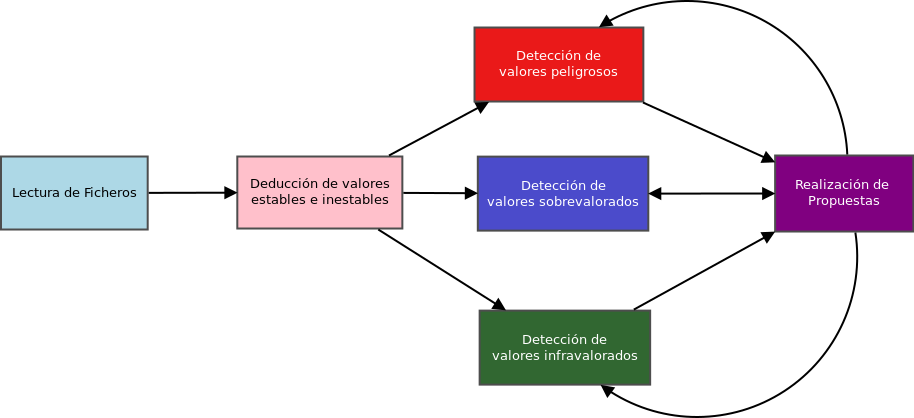
\includegraphics[width=\textwidth]{estructura_bloques}
    \caption{Estructura de los módulos del sistema}
    \label{estructura}
\end{figure}

En la \hyperref[estructura]{Figura \ref*{estructura}} se ve un esquema de los módulos desarrollados, que son:

\begin{description}
    \item[\color{ocre}{Lectura de datos}]: Este es el primer módulo del sistema, en él se han programado reglas para leer los cuatro tipos de ficheros que hay: análisis de empresas, análisis de sectores, cartera del usuario y noticias sobre las empresas y economía.

    \item[\color{ocre}{Deducción de valores}]: Este es el segundo módulo del sistema. En él, se deducen los valores inestables en base a una serie de criterios como el sector de la empresa o las noticias negativas que afectan a una empresa o a su sector. Estos criterios se detallan en la sección Hechos y reglas de cada módulo. Una vez deducidos los valores inestables, se deducen los que son estables en base a las noticias positivas del día.

    \item[\color{ocre}{Detección de valores peligrosos}]: Este es el tercer módulo del sistema. Este módulo sólo afecta a los valores que el usuario tiene en su cartera y se calculan en función de los valores inestables calculados en el módulo anterior.

    \item[\color{ocre}{Detección de valores infravalorados}]: Este módulo puede ejecutase en paralelo junto al anterior. En él se detectan los valores candidatos a ser comprados por el usuario, ya que es posible que su valor ascienda.

    \item[\color{ocre}{Detección de valores sobrevalorados}]: Este módulo también puede ejecutarse en paralelo junto a los dos anteriores. En él se detectan los valores que están demasiado caros, candidatos a que el usuario no los compre o, si posee acciones de alguno de ellos, las venda.

    \item[\color{ocre}{Realización de propuestas}]: Este módulo tiene varias partes: en primer lugar el sistema busca diferentes propuestas para realizar al usuario y calcula el \textit{\textcolor{ocre}{Rendimiento esperado}} de cada una. Después, le muestra al usuario las cinco propuestas con mayor rendimiento esperado y permite que el usuario escoja una. Por último, aplica la propuesta elegida a la cartera del usuario y vuelve a los módulos de detectar valores.
\end{description}

\section{Estructura de funcionamiento del esquema de razonamiento}

El funcionamiento del sistema se aprecia en la \hyperref[estructura]{Figura \ref*{estructura}}, ya que la estructura de módulos utilizada es cada uno de los pasos que realiza el experto. En primer lugar, se realiza la lectura de los datos de entrada. A partir de estos datos, se calculan los valores estables e inestables que hay \textcolor{ocre}{\textbf{en el momento de la ejecución}}. Es importante recalcar esto ya que, según la antigüedad de una noticia buena un valor inestable puede llegar a ser estable durante varios días y viceversa. 

Una vez calculados estos datos, se pasa a detectar valores peligrosos, sobrevalorados e infravalorados y, por último se realizan propuestas al usuario. Estos dos últimos pasos se repiten en bucle hasta que, o bien el sistema se queda sin propuestas o bien el usuario elige salir del programa.

\section{Hechos que el sistema utiliza}

\subsection{Reglas de control}
El sistema tiene una serie de reglas para saber cuándo ejecutar cada módulo del sistema. Estas reglas sirven para poder facilitar la llamada a dicho módulo desde cualquier otro. Estas reglas son:

\begin{enumerate}[\qquad\color{ocre}{$\bullet$}]
    \item Regla para ejecutar el módulo de \textcolor{ocre}{\textit{deducción de valores estables e inestables}}.

    \item Regla para ejecutar el módulo de \textcolor{ocre}{\textit{detección de valores peligrosos, infravalorados y sobrevalorados}}.

    \item Regla para ejecutar el módulo de \textit{\textcolor{ocre}{búsqueda de propuestas}}.
\end{enumerate}

Para \textbf{\textcolor{ocre}{realizar la transición}} de un módulo al siguiente, el sistema utiliza una serie de reglas, para poder controlar la ejecución de los distintos módulos y asegurar de que se termina la ejecución completa de un módulo antes de pasar al siguiente. 

Este tipo de regla se da entre módulo y módulo menos en el caso del módulo de presentación de propuestas, donde primero se buscan propuestas y una vez que hemos encontrado todas las propuestas posibles, buscamos las cinco con máximo rendimiento esperado y se la presentamos al usuario.

\subsection{Reglas de conocimiento global}

También hay reglas para controlar conocimiento global del sistema, estas reglas son:

\begin{enumerate}[\qquad\color{ocre}{$\bullet$}]
    \item Regla para controlar el \textit{\textcolor{ocre}{máximo rendimiento esperado}} encontrado. El valor inicial de esta regla es 0 y se reinicia cada vez que el sistema encuentra una propuesta para el usuario, para poder encontrar la siguiente con mayor rendimiento.

    \item Regla para controlar el \textit{\textcolor{ocre}{número de propuestas}} realizadas al usuario. El valor inicial de esta regla es 0 y se reinicia en cada iteración. Sirve para controlar que, como mucho, se hacen cinco propuestas al usuario.
\end{enumerate}

\section{Hechos y reglas de cada módulo}

\subsection{Deducción de valores estables e inestables}

Las reglas de este módulo son:

\begin{enumerate}[\qquad\color{ocre}{$\bullet$}]
    \item Los valores del sector de la construcción son inestables por defecto.
    \item Si la economía está bajando, los valores del sector servicios son inestables por defecto. 

    Para saber si la economía está bajando, nos fijamos las pérdidas del Ibex en los últimos cinco días.

    \item Si hay una noticia negativa sobre un valor, éste pasa a ser inestable durante dos días.

    En este caso, como el sistema no clasifica el valor como ``inestable durante dos días'' sino que lo deja como inestable porque al usuario le interesan los valores inestables en el momento de la ejecución del programa. Cuando se ejecute el programa a los dos días siguientes dicho valor no se calificará como inestable.

    \item Si hay una noticia negativa sobre un sector, éste pasa a ser inestable durante dos días.

    \item Si hay una noticia negativa sobre la economía, todos los valores pasan a ser inestables durante dos días.

    \item Si hay una noticia positiva sobre un valor o su sector, un valor inestable deja de serlo durante dos días.
\end{enumerate}

Los hechos que se utilizan son las variables de entrada \textit{\textcolor{ocre}{Noticia}}, \textit{\textcolor{ocre}{Empresa}} y \textit{\textcolor{ocre}{Sector}}. Además, para deducir valores estables también se utilizan los hechos de \textit{\textcolor{ocre}{Valor Inestable}}. Por último, también se utiliza un hecho de control para poder llamar al módulo desde los demás módulos.

\subsection{Detección de valores peligrosos, sobrevalorados e infravalorados}

\subsubsection{Detección de valores peligrosos}

Las reglas de este módulo son:

\begin{enumerate}[\qquad\color{ocre}{$\bullet$}]
    \item Si un valor, de la cartera del usuario, es inestable y está perdiendo de forma continua durante los últimos tres días, es peligroso.

    \item Si un valor, de la cartera del usuario, está perdiendo durante los últimos cinco días y la variación en esos días con respecto a la variación del sector es mayor de un 5\%, ese valor es peligroso.
\end{enumerate}

Los hechos que se utilizan son las variables de entrada \textit{\textcolor{ocre}{Cartera del Usuario}} y \textit{\textcolor{ocre}{Empresa}}, ya que el hecho de que un valor tenga una diferencia en la variación con respecto al sector mayor a un 5\% está guardado dentro de la variable empresa. También se utilizan los \textit{\textcolor{ocre}{Valores Inestables}} deducidos anteriormente. 

Por último, se utiliza un hecho de control para acceder al módulo. Éste hecho es el mismo para el módulo de detectar valores peligrosos, infravalorados y sobrevalorados ya que no presentan ninguna dependencia entre sí.

\subsubsection{Detección de valores sobrevalorados}

Las reglas de este módulo son:

\begin{enumerate}[\qquad\color{ocre}{$\bullet$}]
    \item Si una empresa tiene un PER alto y un RPD bajo, dicho valor está sobrevalorado.

    \item Si una empresa es pequeña y tiene el PER alto, entonces dicho valor está sobrevalorado.

    \item Si una empresa es pequeña, tiene un PER mediano y un RPD bajo, entonces dicho valor está sobrevalorado.

    \item Si una empresa es grande, tiene un RPD mediano y un PER alto, entonces dicho valor está sobrevalorado.
\end{enumerate}

Como se ve, el único hecho que necesitamos para calcular valores sobrevalorados es la variable de entrada \textit{\textcolor{ocre}{Empresa}}, que incluye su tamaño, su PER y su RPD. También se utiliza el hecho de control mencionado en el apartado anterior.

Las calificación del PER y del RPD y el tamaño de una empresa se calculan de forma externa al programa y se incluyen en la variable de entrada \textcolor{ocre}{\textit{Empresa}}. 

En el caso del PER su clasificación es:

\begin{enumerate}[\qquad\color{ocre}{$\bullet$}]
    \item Si el PER es $< 12$, entonces es \textbf{\textcolor{ocre}{Bajo}}.
    \item Si el PER es $\geq 12$ y $\leq 18$, entonces es \textbf{\textcolor{ocre}{Mediano}}.
    \item Si el PER es $> 18$, entonces es \textbf{\textcolor{ocre}{Alto}}.
\end{enumerate}

Y en el caso del RPD, su clasificación es:

\begin{enumerate}[\qquad\color{ocre}{$\bullet$}]
    \item Si el RPD es $< 2$, entonces es \textbf{\textcolor{ocre}{Bajo}}.
    \item Si el RPD es $\geq 2$ y $\leq 5$, entonces es \textbf{\textcolor{ocre}{Mediano}}.
    \item Si el RPD es $> 5$, entonces es \textbf{\textcolor{ocre}{Alto}}.
\end{enumerate}

En el caso del tamaño, se clasifica en:

\begin{enumerate}[\qquad\color{ocre}{$\bullet$}]
    \item Si la capitalización supone menos del 2\% del Ibex, entonces es \textbf{\textcolor{ocre}{Pequeña}}.
    \item Si la capitalización está entre el 2\% y el 5\% del Ibex, entonces es \textbf{\textcolor{ocre}{Mediana}}.
    \item Si la capitalización supone más del 5\% del Ibex, entonces es \textbf{\textcolor{ocre}{Grande}}.
\end{enumerate}

\subsubsection{Detección de valores infravalorados}

Las reglas de este módulo son:

\begin{enumerate}[\qquad\color{ocre}{$\bullet$}]
    \item Si una empresa tiene un PER bajo y un RPD alto, la empresa está infravalorada.

    \item Si una empresa ha caído bastante (más de un 30\%) en los últimos 3, 6 o 12 meses, ha subido, pero no mucho en el último mes (es decir, ha subido menos de un 10\%), y el PER es bajo, entonces la empresa está infravalorada.

    \item Si la empresa es grande, tiene un RPD alto y un PER mediano, además no está bajando y se comporta mejor que su sector, entonces la empresa está infravalorada. 

    Se considera que una empresa no está bajando si lleva cinco días sin bajar y se considera que se comporta mejor que su sector si la variación con respecto a éste es mayor al -5\%.
\end{enumerate}

En este módulo se usan los mismos hechos que en el apartado anterior.

\subsection{Realización de propuestas}

Hay cuatro tipo de propuestas que podemos hacerle al usuario: vender un valor peligroso, comprar un valor infravalorado, vender un valor sobrevalorado o cambiar  una acción de la cartera del usuario por otra más rentable. Cada una de estas propuetas tiene una regla asociada:

\begin{enumerate}[\qquad\color{ocre}{$\bullet$}]
    \item \textit{\textcolor{ocre}{Vender valores peligrosos}}: Si una empresa es peligrosa, ha bajado el último mes y ha bajado más de un 3\% respecto a su sector en el último mes, proponer vender las acciones de la empresa. El Rendimiento Esperado de esta propuesta es:

    \begin{theorem}
        \begin{displaymath}
            RE_{valores\;peligrosos} = 20 - 100 \cdot RPD
        \end{displaymath}
    \end{theorem}

    Este rendimiento esperado se debe a que, en la explicación que el sistema da sobre esta propuesta se argumenta que el valor puede caer un 20\% al cabo de un año y, a pesar de que se obtenga el RPD, se perdería 20 - RPD\%.

    \item \textit{\textcolor{ocre}{Invertir en empresas infravaloradas}}: Si una empresa está infravalorada y el usuario tiene dinero para invertir, proponer invertir el dinero en las acciones de la empresa. El Rendimiento Esperado de esta propuesta es:

    \begin{theorem}
        \begin{displaymath}
            RE_{valores\;infravalorados} = \frac{100 \cdot (PER_{medio} - PER)}{5 \cdot PER} + RPD
        \end{displaymath}
    \end{theorem}

    Este rendimiento esperado se debe a que, en la explicación que el sistema da sobre esta propuesta, se argumenta que el PER de la empresa tenderá al PER medio del sector en 5 años, por lo que en un año el usuario obtendría la resta entre el PER medio del sector y el PER de la empresa, divido entre 5 por el valor actual del PER añadiéndole los beneficios por dividendos.

    \item \textit{\textcolor{ocre}{Vender valores sobrevalorados}}: Si una empresa de la cartera del usuario está sobrevalorada y el rendimiento por año es $< 5 + precio\;dinero$, proponer vender las acciones de la empresa. El Rendimiento Esperado de esta propuesta es:

    \begin{theorem}
        \begin{displaymath}
            RE_{valores\;sobrevalorados} = -RPD + \frac{100 \cdot (PER_{medio} - PER)}{5 \cdot PER}
        \end{displaymath}
    \end{theorem}

    Este rendimiento esperado se debe a que, en la explicación que el sistema da sobre esta propuesta, se argumenta que el PER de la empresa bajará al PER medio del sector en unos cinco años, por tanto, perderíamos loos beneficios por dividendos pero ganaríamos la diferencia entre el valor actual del PER menos la media del sector entre cinco por el valor actual del PER.

    \item \textit{\textcolor{ocre} {Cambiar valores de la cartera por otros más rentables}}: Si una empresa, $E_1$, no está sobrevalorada y su RPD es mayor que la $revalorización\;por\;semestre +1$  de una empresa de la cartera del usuario, $E_2$, que no está infravalorada, proponer cambiar las acciones de $E_2$ por las de $E_1$. El Rendimiento Esperado de esta propuesta es:

    \begin{theorem}
        \begin{displaymath}
            RE_{cambiar\;valores} = RPD_1 - (Revalorizaci\acute{o}n\;Semestre_2 + RPD_2 + 1)
        \end{displaymath}
    \end{theorem}

    Este rendimiento esperado se debe a que, en la explicación que el sistema da sobre esta propuesta, se argumenta que $E_1$ debe de darnos un $RPD_1$, que es más de lo que obtendría el usuario con $E_2$ al cabo de un semestre. El sumar un 1 al final es debido al coste de realizar el cambio.
\end{enumerate}

Estas reglas usan las variables de entrada \textit{\textcolor{ocre}{Empresa}}, \textit{\textcolor{ocre}{Cartera del usuario}} y los valores detectados anteriormente como \textit{\textcolor{ocre}{sobrevalorados}}, \textit{\textcolor{ocre}{infravalorados}} y \textit{\textcolor{ocre}{peligrosos}}. Por último, también se usa un hecho de control para controlar las llamadas a este módulo desde el resto.

% Dentro de este módulo también se incluyen las reglas para manejar la I/O con el usuario, pero no van a ser explicadas en esta memoria debido a que ésta no está enfocada a dar tantos detalles sobre implementación.

\chapterimage{chapter_head_5}
\chapter{Breve manual de uso del sistema}

Para poder usar el programa, es necesario disponer de \textbf{\textcolor{ocre}{CLIPS}} instalado en el ordenador. Una vez lo tengamos instalado, tecleamos en la consola de CLIPS los siguientes comandos:

\begin{verbatim}
> (load inversor.clp)

> (reset)

> (run)
\end{verbatim}

Tras esto aparecerán cinco o menos opciones, junto a un número a la izquierda, de la siguiente forma:

\begin{verbatim}
1 Propuesta uno
2 Propuesta dos
3 Propuesta tres
4 Propuesta cuatro
5 Propuesta cinco
6 No, he acabado
¿Quieres aplicar alguno de estos consejos? Selecciona el número
\end{verbatim}

El usuario debe introducir el número correspondiente a la opción deseada. La última opción es para cerrar el programa y el resto, propuestas acompañadas junto a una explicación y el rendimiento esperado.

\end{document}